\subsection{Statistical Model Selection via Argumentation}

\label{sub:statistical_model_selection}

The foundation of this MSc Project is the paper \cite{sassoon2014}. The following papers of Sassoon \textit{et al.} \cite{sassoon2016,sassoon2016CD} have been as well taken into account, as they provide an elegant solution to express the order of preferences in different \glspl{CD}.

The goal of this project is to use Argumentation Theory for Statistical Model Selection in mostly clinical environments. The demand into systems that support clinicians in the analysis of this data in their day-to-day practice is extending (because of increasing availability, growing size of datasets available for clinicians, and raising awareness on evidence based decision making extend). In the following section a short summary on the paper will be given. 

To overcome the issue of clinicians analysing data and models on their compatibility \cite{sassoon2014} proposes an approach of an intelligent model selection system which is capable of suggesting appropriate model(s) to a clinician during the design stage of a study, taking in account the research question, the clinical data and any external relevant input and preferences. In addition this system should be able to support its decision by providing the argumentation for and against a model to the user. As clinicians might not always be qualified to perform the statistical analysis required for their research question, the process of designing models, specifying its requirements and providing the arguments for or agains these models should be separated from the actual design process and be done by a statistician. The statistician is thereby in charge of understanding the data in the context of the research question and provide arguments that are able to recommend the best suited statistical analysis for a particular research question. 

Furthermore  Sassoon \textit{et al.} address the problem of defeasible knowledge, as the (counter-) arguments for a model are often contradicting and the system, the clinician and the statistician might have some preferences for one or the other model. Therefore they propose to split the problem into two parts (i) a (defeasible) \textit{knowledge base} that contains the statistical model definitions, the objectives and assumptions of a model; (ii) \textit{argumentation schemes} to guide the model selection process and to represent expressed preferences. In the later papers \cite{sassoon2016,sassoon2016CD} they propose to reflect this by \gls{CD} specific preference orders that are ordered themselves by a priority.

The \textit{knowledge base} is used to instantiate the \textit{argumentation schemes}. The knowledge base itself defines how research objectives can be achieved through different statistical models considering their given assumptions. \textit{Research objectives} are defined as different 'families' of analysis (e.g. survival analysis or categorical outcome variable analysis).


\glsreset{SKB}
\subsubsection*{Statistical Knowledge Base}


The \gls{SKB} consists of objectives $\O=\{o_1, ..., o_u\}$ (different types of research questions), models $\M=\{m_1, ..., m_v\}$ and assumptions $\A = \{a_1, ..., a_w\}$. Models represent statistical analysis techniques employable to answer a research question. Assumptions are conditions that ought to be met to employ a model.

\begin{definition}
	Let $R_{\O\M}: \O \times \M$ be a m:n\footnote{Each objective can be achieved by one or more models, each model can answer one or more objectives.}-relationship such that $(o_i, m_j)\in R_{\O\M}$ implies objective $o_i$ can be achieved by means of model $m_j$. 
\end{definition}

\begin{definition}
	Let $R_{\M\A}: \M \times \A$ be relation between models and their assumptions. $(m_i, a_j)\in R_{\M\A}$ implies  the model $m_i$ requires the assumption $a_j$ to be true to be applicable. Let $\A(m_i) = \{a_j | (m_i, a_j) \in R_{\M\A}\}$ be the set of assumptions of $m_i$.
\end{definition}

\begin{remark}
In contradiction to \cite{sassoon2014} we will not use the proposed approach to distinguish between \textit{critical} and \textit{non-critical} assumptions, as they have been used in the initial approach to express the preference over different possible models. However, all assumptions assigned to one model have to hold to make a model possible. Instead we gonna use the \gls{CD}-driven approach described in \cite{sassoon2016CD}.
\label{rem:cds}
\end{remark}


\begin{definition}
To apply a model $m_i$ all assumptions $\A(m_i) = \{a_j | (m_i, a_j) \in R_{\M\A} \}$ must be met\footnote{As described in \autoref{rem:cds} we regard all assumptions as critical.}.
\end{definition}

Each \textit{assumption} will be either specified as a specific property of the data set (assessed by applying tests on the data set) or as a characteristic of the population of interest or the way in which the data set was collected from that population (relying on the expertise of a domain expert). Sassoon proposes a partitioning of all assumptions: $\A_t$ denotes the set of tests (and apply a test on the available data set). $\A_q$ denotes the set of queries (and will be assessed by asking the clinician for an opinion). Lets define $\A_t(m_i)= \{a_j| (m_i, a_j) \in \A_t\}$ and $\A_q(m_i)= \{a_j| (m_i, a_j) \in \A_q\}$. Note that critical assumptions can be in either $\A_t$ or $\A_q$: $ R_{\M\A} = \A_q \cup \A_t, ~\A_q \cup \A_t = \emptyset$. 

The \autoref{fig:skb_example} shows the structure between \textit{objectives}, \textit{models} and \textit{assumptions} in a small example. The assumptions $\{a_1, a_2, a_3\} \in \A_t$ are based on the provided data set, $\{a_3, a_5\} \in \A_q$ are based on the domain expertise. Objectives $\{o_1, o_2\}$ can  be achieved by the possible model $m_1$, $o_3$ can only be achieved by $m_3$. Note that $m_3$ is still a possible model although the non critical assumption $a_4$ doesn't hold.

\begin{figure}[h]
\centering
\begin{tikzpicture}[->,>=stealth',shorten >=1pt,auto,node distance=1cm,
                    thick]

  \node[main] (o1) {$o_1$};
  \node[main] (o2) [below of=o1] {$o_2$};
  \node[main] (o3) [below of=o2] {$o_3$};

  \node[main,n_fill_green] (m1) [right= 1.5cm of o1] {$m_1$};
  \node[main,n_fill_red] (m2) [below of=m1] {$m_2$};
  \node[main,n_fill_green] (m3) [below of=m2] {$m_3$};

  \node[main, double,n_fill_red] (a2) [right= 1.5cm of m1] {$a_2$};  
  \node[main,n_fill_green] (a1) [above of=a2] {$a_1$};
  \node[main, double,n_fill_green] (a3) [below of=a2] {$a_3$};
  \node[main,n_fill_red] (a4) [below of=a3] {$a_4$};
  \node[main, double,n_fill_green] (a5) [below of=a4] {$a_5$};
  
  \node (DB) [cylinder, shape border rotate=90,draw,minimum height=2cm,minimum width=1.3cm, fill=gray!10][right= 3cm of a2]{DB};
  \node (T) [draw=black,fill=gray!10,cloud,font=\fontfamily{ppl}\fontsize{1cm}{1.5cm}\selectfont][right= 3cm of a4]{?};
  
  \path[every node/.style={font=\sffamily\small}]
    (a1) edge [] node [left] {} (m1)
         edge [] node [left] {} (m2)
    (a2) edge [] node [left] {} (m2)
    (a3) edge [] node [left] {} (m2)
    (a4) edge [] node [left] {} (m2)
         edge [dashed] node [left] {} (m3)
         edge [] node [left] {} (m3)
    (a5) edge [] node [left] {} (m3)
    (m1) edge [] node [left] {} (o1)
         edge [] node [left] {} (o2)
	(m2) edge [] node [left] {} (o1)
	     edge [] node [left] {} (o2)
	(m3) edge [] node [left] {} (o3)
	(DB) edge [] node [left] {} (a1)
         edge [] node [left] {} (a2)
         edge [] node [left] {} (a4)
         edge [] node [left] {} (a1)
    (T)  edge [] node [left] {} (a3)
         edge [] node [left] {} (a5)
    ;
\end{tikzpicture}
\caption{Example of a \gls{SKB}. Double circled assumptions represent critical assumptions. Green coloured assumptions hold while red coloured assumptions do not hold. Green coloured models are the possible models.}
\label{fig:skb_example}
\end{figure}



\subsubsection*{Different Processes to instantiate Arguments from the Knowledge Base}

To achieve an objective $o_c$ (which has been selected by the clinician) a number of models $m_i$ might be possible providing all their assumptions $\A(m_i)$ are met. The process of instantiating the arguments can be seen in AS\autoref{as:1}.

\begin{AS}[h]
\centering
	\caption{Constructed argument for a Possible Model.\label{as:1}}
	\fbox{\begin{minipage}{0.7\textwidth}
	\begin{itemize}
		\item Model $m_i$ achieves objective $o_c$.
		\item The data set meets the set of assumptions $\A_t' = \A_t(m_i)$.
		\item The research project meets the set of assumptions $\A_q' = \A_q(m_i)$.
		\item $\A(m_i) \subseteq \A_t' \cup \A_q'$.
	\end{itemize}
	\rule{\textwidth}{0.5pt}\\
	$~~~~\Rightarrow$  $m_i$ is a possible model for the research question $o_c$.
	\end{minipage}}
\end{AS}

As quoted in \autoref{rem:cds} we will not use the inital approach of instantiating AS2 as described in \cite{sassoon2014} but the \gls{CD}-based approach described in \cite{sassoon2016CD}.

To express the preferences for one model over another, Sassoon \textit{et al.} \cite{sassoon2016} propose to use the \glspl{EAF} \cite{Modgil2009} approach. These modifications enable argumentation on preferences which are encapsulated as arguments, therefore we will be able to consider conflicting preferences in our system and ensure scalability and express orders of importance between statistical reasons to prefer one model over another and clinician's preferences in specific contexts.

Sassoon \textit{et al.} suggest in their latest paper \cite{sassoon2016CD} how an \gls{EAF} can be employed to capture and reason with statistical and research domain knowledge that affects the relative strength of arguments and thereby implies an order over different context domains. To do so, \glspl{CPAF} are used in combination with \glspl{EAF} by defining a preference ordering $Pref : \M \times \M$ for a given set of models $\M = \{m_1, ..., m_n\}$ by assigning performance measurements to each model for a given \gls{CD}. A sample performance function for model resilience to censoring (CD1) can be seen in \autoref{tab:cd1}, an additional second performance function for based on the intention of the model (CD2) can be seen in \autoref{tab:cd2}.
\begin{table}[t]
	\centering
	\begin{tabular}{|l|c|l|c|}
	\hline
	Context Domain 			& Model 			& Performance measure & Order\\
	\hline\hline
	\multirow{3}{*}{absent} & $m_1$ KM 		& unaffected		& 	\multirow{3}{*}{$m_1, m_2, m_3$}\\
							& $m_2$ PH		& unaffected		&\\
							& $m_3$ $X^2$	& unaffected		&\\
	\hline
	\multirow{3}{*}{light} 	& $m_1$ KM 		& unaffected		& \multirow{3}{*}{$m_3 \prec m_1, m_2$}\\
							& $m_2$ PH		& unaffected		&\\
							& $m_3$ $X^2$	& affected		&\\
	\hline
	\multirow{3}{*}{heavy} 	& $m_1$ KM 		& affected		& \multirow{3}{*}{$m_1, m_3 \prec m_2$}\\
							& $m_2$ PH		& unaffected		&\\
							& $m_3$ $X^2$	& affected		&\\
	\hline
	\end{tabular}
	\caption{Sample performance function for model resilience to censoring (CD1) \cite{sassoon2016CD}}
	\label{tab:cd1}
\end{table}


\begin{table}[b]
	\centering
	\begin{tabular}{|l|c|l|c|}
	\hline
	Context Domain 			& Model 			& Performance measure & Order\\
	\hline\hline
	\multirow{3}{*}{predict}& $m_1$ KM 		& avoid		& \multirow{3}{*}{$m_1, m_3 \prec m_2$}\\
							& $m_2$ PH		& suitable	&\\
							& $m_3$ $X^2$	& avoid		&\\
	\hline
	\multirow{3}{*}{explain}& $m_1$ KM 		& suitable	& \multirow{3}{*}{$m_1, m_2 \prec m_3$}\\
							& $m_2$ PH		& suitable	&\\
							& $m_3$ $X^2$	& neutral	&\\
	\hline
	\end{tabular}
	\caption{Sample performance function for model intent (CD2) \cite{sassoon2016CD}}
	\label{tab:cd2}
\end{table}
These orders over the models can then be transferred into preference arguments. \autoref{tab:cd1} and \ref{tab:cd2} could be translated into the set of the following preference arguments:

\begin{align*}
CD1_{light} &\twoheadrightarrow (m_3 \rightarrow m_1)\\
CD1_{light} &\twoheadrightarrow (m_3 \rightarrow m_2)\\
CD1_{heavy} &\twoheadrightarrow (m_1 \rightarrow m_2)\\
CD1_{heavy} &\twoheadrightarrow (m_3 \rightarrow m_2)\\
\\
CD2_{predict} &\twoheadrightarrow (m_1 \rightarrow m_2)\\
CD2_{predict} &\twoheadrightarrow (m_3 \rightarrow m_2)\\
CD2_{explain} &\twoheadrightarrow (m_1 \rightarrow m_3)\\
CD2_{explain} &\twoheadrightarrow (m_2 \rightarrow m_3)\\
\end{align*}


\begin{figure}[b!]
\centering
\begin{tikzpicture}[->,>=stealth',shorten >=1pt,auto,node distance=3cm,
                    thick]
  	\node[main] (m1) {$m_1$};
	\node[main] (m2) [below left of=m1]{$m_2$};
	\node[main] (m3) [below right of=m1]{$m_3$};

  \path[every node/.style={font=\sffamily\small}]
    (m1) edge [bend right] coordinate [pos=0.5] (m1m2) node [left] {} (m2)
    (m1) edge [] coordinate [pos=0.5] (m1m3) node [left] {} (m3)
    (m2) edge [] coordinate [pos=0.5] (m2m1) node [left] {} (m1)
    (m2) edge [bend right] coordinate [pos=0.5] (m2m3) node [left] {} (m3)
    (m3) edge [bend right] coordinate [pos=0.5] (m3m1) node [left] {} (m1)
    (m3) edge [] coordinate [pos=0.5] (m3m2) node [left] {} (m2)
    ;
	\node[box] (CD1light1)[above right of=m3m1,xshift=-1cm,yshift=-1cm] {$CD1_{light}$};
	\node[box] (CD1light2)[below of=m3m2, yshift=1cm] {$CD1_{light}$};  
    
   \path [every node/.style={red}] 
   (CD1light1) edge [->>] node [left] {} (m3m1)
   (CD1light2) edge [->>] node [left] {} (m3m2)
   ;
\end{tikzpicture}
\caption{\gls{EAF} including the preference attacks that are generated if $CD1_{light}$ holds. The attacks between the possible models between $(m_3,m_2)$ and $(m_3,m_1)$ are canceled out and $m_3$ remains as possible model after applying the preference $CD1$ where $light$ was measured as performance measure.}
\label{fig:eaf_intro}
\end{figure}


Sassoon \textit{et al.} propose further to assign each \gls{CD} a priority, so that they get evaluated one after the other, until one final (if at all possible) preferred model remains. After evaluating the possible models by using \autoref{as:1} we will form an \gls{AF} where each of the possible model attacks every other model. Then each \gls{CD} will be initiated and add its attacks on the existing \gls{AF}. After that, the \gls{EAF} will be evaluated w.r.t. the argument holding in this \gls{CD} $\S_1'$ (e.g. $\S_1' = \{CD1_{heavy}\}$). If a final decision (only one model is acceptable w.r.t. $\S_1'$) can be made, the process terminates. Otherwise the next \gls{CD} gets evaluated (e.g. $\S_2' = \{CD2_{predict}\}$). This is continued until no further preferences are defined or only one -- the preferred -- model remains. The overall process can be seen in \autoref{lst:preferences_process}.

During this process the \glspl{CD} that relate to statistical theory are regarded as more important (lower priority) than clinician preferences. This is reflected in the final web application by reserving the priorities lower than 10 to the statistician only. Clinicians can express their personal preferences in \glspl{CD} with a priority higher than or equal to 10. 
 
\todo{Write pseudocode}
\begin{algorithm}[h]
\caption{My algorithm}\label{lst:preferences_process}
\begin{algorithmic}[1]
\Procedure{GetPreferredModel}{RQ: ResearchQuestion, DS: Dataset}
\State $possibleModels \gets \{m_i : m_i \in RQ.models~\&~ m_i\text{ is possible in accordance \autoref{as:1}} \}$
\If {$i > \textit{stringlen}$} \Return false
\EndIf
\State $j \gets \textit{patlen}$
\State \emph{loop}:
\If {$\textit{string}(i) = \textit{path}(j)$}
\State $j \gets j-1$.
\State $i \gets i-1$.
\State \textbf{goto} \emph{loop}.
\State \textbf{close};
\EndIf
\State $i \gets i+\max(\textit{delta}_1(\textit{string}(i)),\textit{delta}_2(j))$.
\State \textbf{goto} \emph{top}.
\EndProcedure
\end{algorithmic}
\end{algorithm}

\todo{include generated AF after AS 1, CD1, CD2}
\todo{Source by isabel for pic below}
\begin{figure}[h]

\centering
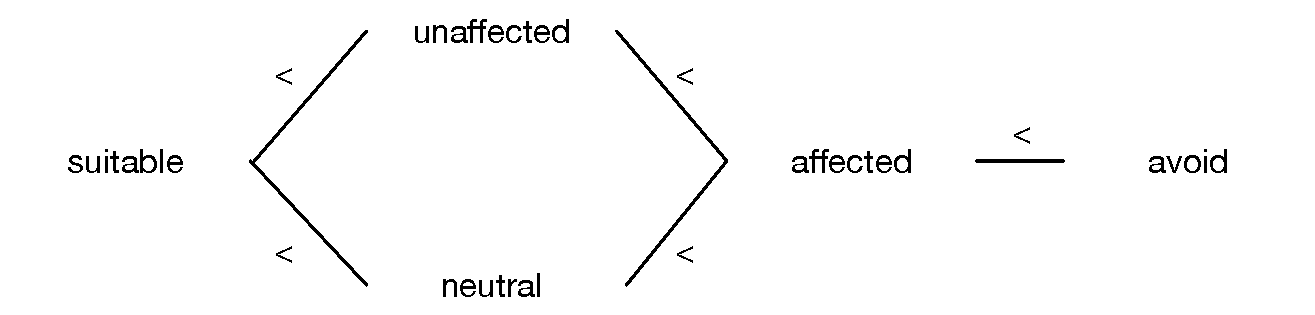
\includegraphics[width=0.8\textwidth]{figures/order_context_domain}
\caption{Order of different results in context domains }
\end{figure}

